\documentclass[aspectratio=169]{beamer}
\usepackage{../downey_format_slides}



\usefonttheme{serif}
\setbeamercolor{normal text}{fg=black}

% Make all structural text black (titles, sections, etc.)
\setbeamercolor{structure}{fg=black}

% Frame titles (top title)
\setbeamercolor{frametitle}{fg=black}

% Figure caption ("Figure:")
\setbeamercolor{caption name}{fg=black}
\setbeamercolor{caption}{fg=black}

% Section titles in footer/header
\setbeamercolor{section in head/foot}{fg=black}

% Just in case
\setbeamercolor{title}{fg=black}


% --- Theme setup (minimal) ---
\usetheme{default}
\useoutertheme{default}
\useinnertheme{default}

% Remove navigation symbols
\setbeamertemplate{navigation symbols}{}

% Define your red
% \definecolor{myred}{RGB}{225,120,120}
\definecolor{myred}{RGB}{115,0,10}


\usepackage{color} % color added for editing
\newcommand{\bl}[1]{\textcolor[rgb]{0.00,0.00,1.00}{#1}}
\newcommand{\gr}[1]{\textcolor[rgb]{0.00,0.50,0.00}{#1}}
\newcommand{\rd}[1]{\textcolor[rgb]{0.75,0.00,0.00}{#1}}
\newcommand{\tl}[1]{\textcolor[rgb]{0,0.6,0.60}{#1}}

\usepackage{booktabs}
\usepackage{bm}
\usepackage{mdframed}
\usepackage{xcolor}

% --- Custom footline ---
\setbeamertemplate{footline}{
\leavevmode

% Thin red line (moved to TOP)
\begin{beamercolorbox}[wd=\paperwidth,ht=0.1ex]{}
\color{myred}\rule{\paperwidth}{0.1ex}
\end{beamercolorbox}

\hbox{
\begin{beamercolorbox}[wd=\paperwidth,ht=2.5ex,dp=1ex]{}
\hspace{1em}
\insertsection
\hfill
\insertframenumber{} / \inserttotalframenumber
\hspace{1em}
\end{beamercolorbox}
}
}

% Remove headline entirely
\setbeamertemplate{headline}{}

% Optional: clean fonts
\setbeamerfont{footline}{size=\small}







\title{Chapter~7~Support Vector Machines}
\author{Austin R.J. Downey}
\date{}

\begin{document}

\section{Machine Learning for Engineering Problem Solving}
\frame{\titlepage}


\section{Chapter~7~Support Vector Machines}


%------------------------------------------------

%------------------------------------------------

\begin{frame}{Support Vector Machines}
\begin{columns}

\column{0.42\textwidth}

Support Vector Machines are geometric classifiers.

\vspace{0.5em}

Key idea:
\begin{itemize}
\item Separate classes with a decision boundary
\item Maximize the margin around that boundary
\item Use nearby points to define the boundary
\end{itemize}

\vspace{0.5em}

Those nearby points are called:

\[
\textbf{Support Vectors}
\]

\column{0.58\textwidth}
\centering

\includegraphics[width=\textwidth]{../figures/SVM_large_margin_classification}

\vspace{0.3em}
Large margin classification.

\end{columns}
\end{frame}

%------------------------------------------------

\begin{frame}{Large Margin Classification}
\begin{columns}

\column{0.42\textwidth}

Many linear classifiers may separate the training data.

\vspace{0.5em}

SVMs choose the classifier that creates the widest possible margin.

\vspace{0.5em}

This margin is often called the:

\[
\text{street}
\]

\vspace{0.5em}

Only points on the edge of the street directly affect the boundary.

\column{0.58\textwidth}
\centering

\includegraphics[width=\textwidth]{../figures/SVM_large_margin_classification}

\vspace{0.3em}
The boundary is shaped by the support vectors.

\end{columns}
\end{frame}

%------------------------------------------------

\begin{frame}{SVMs Need Feature Scaling}
\begin{columns}

\column{0.42\textwidth}

SVMs are sensitive to feature scale.

\vspace{0.5em}

If one feature dominates the scale, the margin may be distorted.

\vspace{0.5em}

A common preprocessing step is:

\[
\texttt{StandardScaler}
\]

\vspace{0.5em}

Scaling usually produces a more appropriate decision boundary.

\column{0.58\textwidth}
\centering
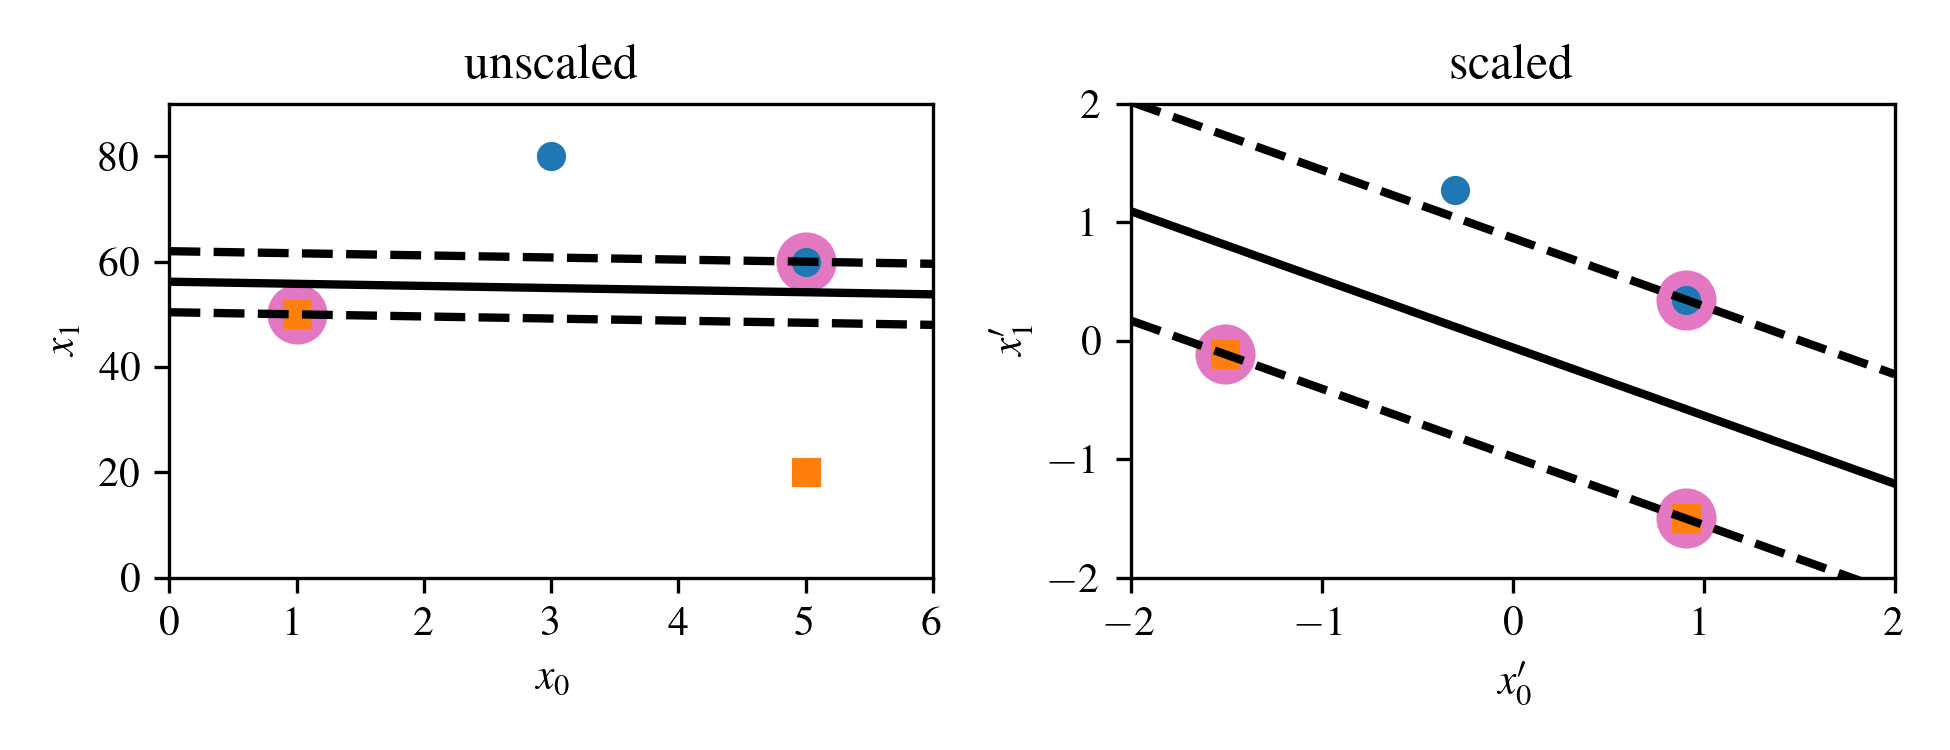
\includegraphics[width=\textwidth]{../figures/SVM_feature_scaling}

\vspace{0.3em}
Effect of feature scaling.

\end{columns}
\end{frame}

%------------------------------------------------

\section{7.1~Linear SVM Classification}

\begin{frame}{Hard Margin Classification}
\begin{columns}

\column{0.42\textwidth}

Hard margin classification requires:

\begin{itemize}
\item All points correctly classified
\item No margin violations
\end{itemize}

\vspace{0.5em}

Limitations:
\begin{itemize}
\item Only works for linearly separable data
\item Very sensitive to outliers
\end{itemize}

\vspace{0.5em}

A single outlier can make the hard-margin problem impossible or unstable.

\column{0.58\textwidth}
\centering

\includegraphics[width=\textwidth]{../figures/SVM_hard_margin.png}

\vspace{0.3em}
Hard margin sensitivity to outliers.

\end{columns}
\end{frame}

%------------------------------------------------

\begin{frame}{Soft Margin Classification}
\begin{columns}

\column{0.42\textwidth}

Soft margin classification allows some margin violations.

\vspace{0.5em}

Goal:
\begin{itemize}
\item Keep the margin wide
\item Limit classification errors
\item Improve generalization
\end{itemize}

\vspace{0.5em}

The balance is controlled by:

\[
C
\]

\vspace{0.5em}

Smaller \(C\) gives stronger regularization.

\column{0.58\textwidth}
\centering
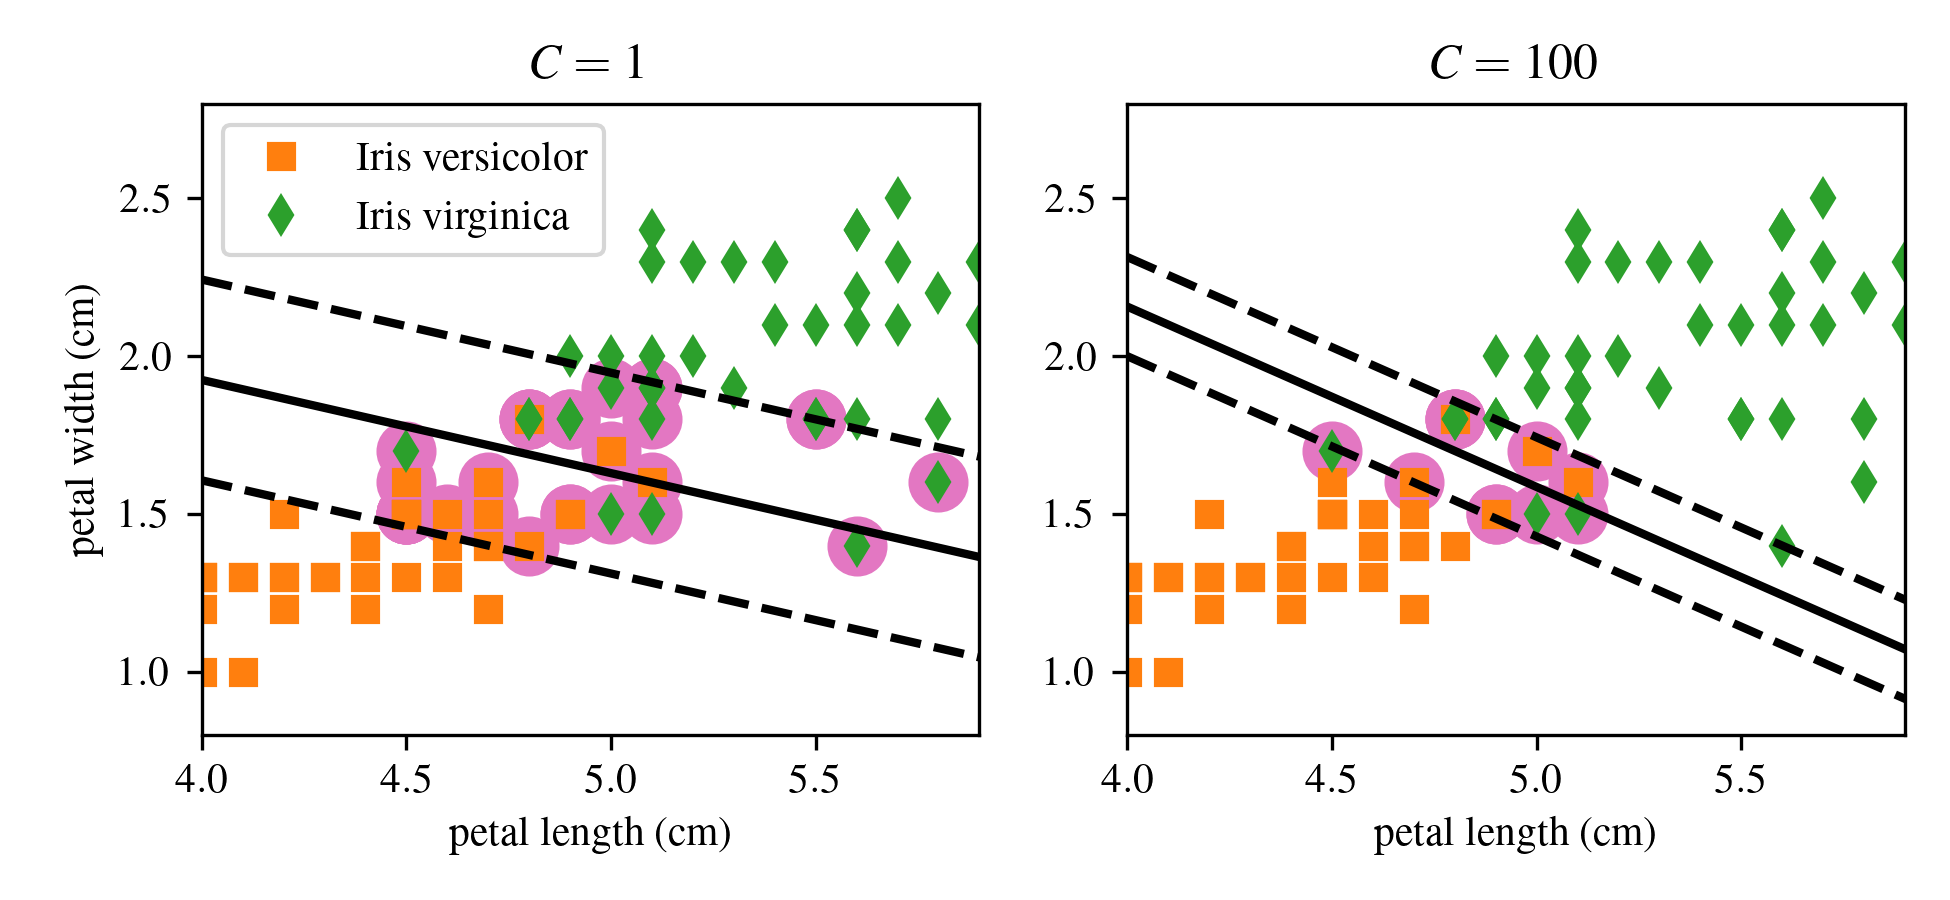
\includegraphics[width=\textwidth]{../figures/SVM_hyperparameter_C.png}

\vspace{0.3em}
Effect of the \(C\) hyperparameter.

\end{columns}
\end{frame}

%------------------------------------------------

\begin{frame}{The Role of \(C\)}

The hyperparameter \(C\) controls the tradeoff between margin width and violations.

\vspace{0.75em}

\begin{itemize}
\item Smaller \(C\):
\begin{itemize}
\item Wider margin
\item More violations allowed
\item More regularization
\end{itemize}

\vspace{0.5em}

\item Larger \(C\):
\begin{itemize}
\item Narrower margin
\item Fewer violations allowed
\item Less regularization
\end{itemize}
\end{itemize}

\vspace{0.75em}

\begin{exampleblock}{Note}
Overfitting in an SVM can often be reduced by decreasing \(C\).
\end{exampleblock}

\end{frame}

%------------------------------------------------

\begin{frame}{SVM Notation}

In earlier chapters, model parameters were often written as:

\[
\boldsymbol{\theta}
\]

\vspace{0.5em}

For SVMs, we usually write:

\[
\mathbf{w}
\quad \text{and} \quad
b
\]

\vspace{0.5em}

where:

\begin{itemize}
\item \(\mathbf{w}\): weight vector
\item \(b\): bias term
\item No extra bias feature \(x_0=1\) is appended
\end{itemize}

\vspace{0.5em}

The decision function is built directly from \(\mathbf{w}\), \(\mathbf{x}\), and \(b\).

\end{frame}

%------------------------------------------------

\begin{frame}{Decision Function and Predictions}

A linear SVM computes:

\[
\mathbf{w}^{\top}\mathbf{x}+b
=
w_1x_1+\cdots+w_nx_n+b
\]

\vspace{0.5em}

Prediction rule:

\[
\hat{y}
=
\begin{cases}
0 & \text{if } \mathbf{w}^{\top}\mathbf{x}+b < 0\\
1 & \text{if } \mathbf{w}^{\top}\mathbf{x}+b \ge 0
\end{cases}
\]

\vspace{0.5em}

The decision boundary occurs when:

\[
\mathbf{w}^{\top}\mathbf{x}+b = 0
\]

\end{frame}

%------------------------------------------------

\begin{frame}{SVM Decision Function}
\begin{columns}

\column{0.42\textwidth}

For two features, the decision function is a plane.

\vspace{0.5em}

Important levels:
\[
h=0
\]
defines the decision boundary.

\[
h=1
\quad \text{and} \quad
h=-1
\]
define the margin boundaries.

\vspace{0.5em}

Training adjusts \(\mathbf{w}\) and \(b\) to make the margin wide.

\column{0.58\textwidth}
\centering
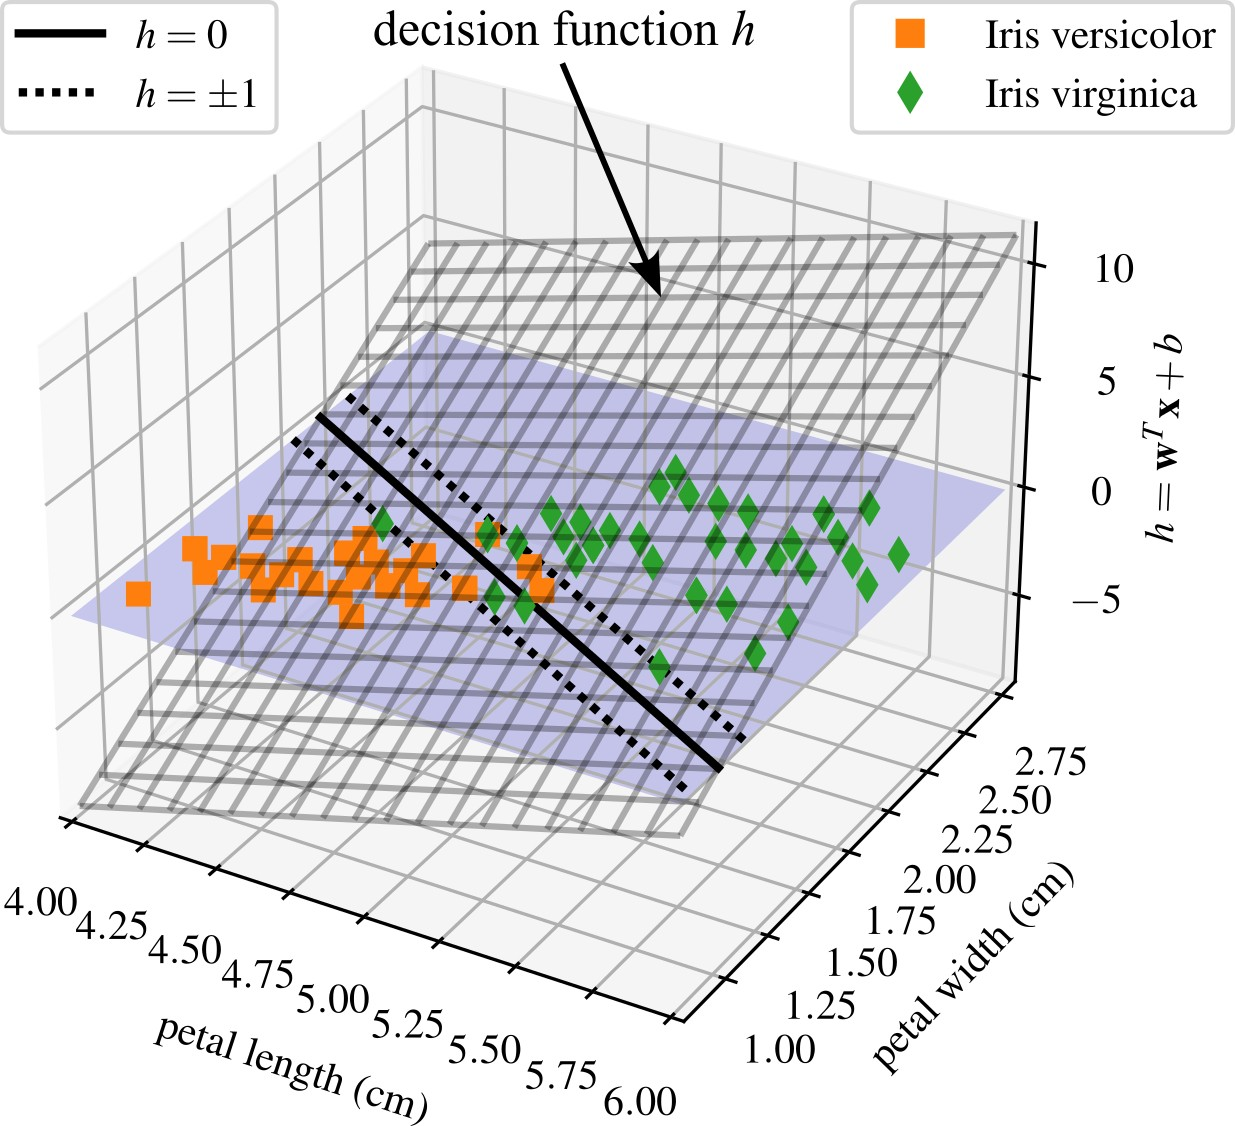
\includegraphics[width=\textwidth]{../figures/SVM_decision_function}

\vspace{0.3em}
Decision function for the Iris dataset.

\end{columns}
\end{frame}

%------------------------------------------------

\begin{frame}{Training Objective}
\begin{columns}

\column{0.42\textwidth}

The slope of the decision function depends on:

\[
\lVert \mathbf{w}\rVert
\]

\vspace{0.5em}

Reducing \(\lVert \mathbf{w}\rVert\) increases the margin.

\vspace{0.5em}

Therefore, SVM training tries to:

\[
\text{minimize } \lVert \mathbf{w}\rVert
\]

\vspace{0.5em}

This maximizes the margin between classes.

\column{0.58\textwidth}
\centering
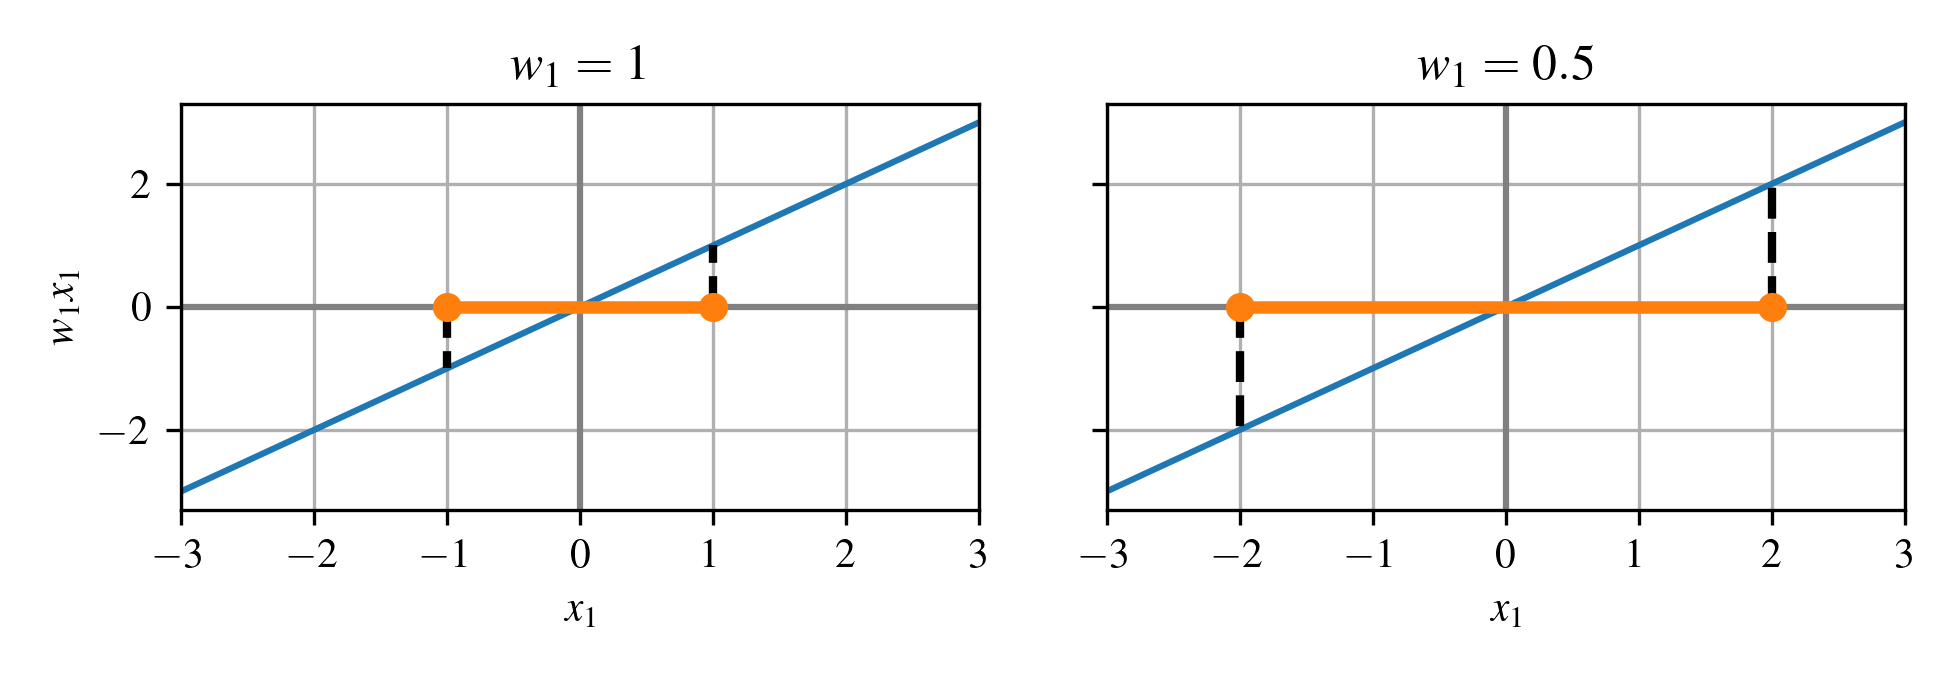
\includegraphics[width=\textwidth]{../figures/SVM_weight_vectors}

\vspace{0.3em}
Smaller weights produce a larger margin.

\end{columns}
\end{frame}

%------------------------------------------------

\begin{frame}{Hard Margin Objective}

Let \(t^{(i)}=-1\) for negative samples and \(t^{(i)}=1\) for positive samples.

\vspace{0.5em}

The hard margin constraint is:

\[
t^{(i)}
\left(
\mathbf{w}^{\top}\mathbf{x}^{(i)}+b
\right)
\ge 1
\]

\vspace{0.5em}

The optimization problem is:

\[
\begin{split}
& \underset{\mathbf{w}, b}{\text{minimize}}
\quad
\frac{1}{2}\mathbf{w}^{\top}\mathbf{w} \\
& \text{subject to}
\quad
t^{(i)}
\left(
\mathbf{w}^{\top}\mathbf{x}^{(i)}+b
\right)
\ge 1
\end{split}
\]

\vspace{0.5em}

This enforces a margin with no violations.

\end{frame}

%------------------------------------------------

\begin{frame}{Why Minimize \(\frac{1}{2}\mathbf{w}^{\top}\mathbf{w}\)?}

The objective

\[
\frac{1}{2}\mathbf{w}^{\top}\mathbf{w}
\]

is equivalent to

\[
\frac{1}{2}\lVert \mathbf{w}\rVert^2
\]

\vspace{0.5em}

Why use the squared norm?

\begin{itemize}
\item It is smooth and differentiable
\item Its derivative is simple
\item It makes optimization easier
\end{itemize}

\vspace{0.5em}

\begin{exampleblock}{Note}
Minimizing \(\lVert \mathbf{w}\rVert\) directly is harder because it is not differentiable at \(\mathbf{w}=0\).
\end{exampleblock}

\end{frame}

%------------------------------------------------

\begin{frame}{Soft Margin Objective}

Soft margin classification introduces slack variables:

\[
\zeta^{(i)} \ge 0
\]

\vspace{0.5em}

Each \(\zeta^{(i)}\) measures how much sample \(i\) violates the margin.

\vspace{0.5em}

The optimization problem becomes:

\[
\begin{split}
& \underset{\mathbf{w}, b, \zeta}{\text{minimize}}
\quad
\frac{1}{2}\mathbf{w}^{\top}\mathbf{w}
+
C\sum_{i=1}^{m}\zeta^{(i)}
\\
& \text{subject to}
\quad
t^{(i)}
\left(
\mathbf{w}^{\top}\mathbf{x}^{(i)}+b
\right)
\ge
1-\zeta^{(i)}
\end{split}
\]

\vspace{0.5em}

The parameter \(C\) controls the penalty for violations.

\end{frame}

%------------------------------------------------

\begin{frame}{Quadratic Programming}

Both hard-margin and soft-margin SVMs are convex quadratic optimization problems.

\vspace{0.5em}

General quadratic programming form:

\[
\begin{split}
& \underset{\mathbf{p}}{\text{minimize}}
\quad
\frac{1}{2}\mathbf{p}^{\top}\mathbf{H}\mathbf{p}
+
\mathbf{f}^{\top}\mathbf{p}
\\
& \text{subject to}
\quad
\mathbf{A}\mathbf{p}\le \mathbf{b}
\end{split}
\]

\vspace{0.5em}

For a linear SVM:

\begin{itemize}
\item \(\mathbf{p}\) contains the weights and bias
\item The objective encodes margin maximization
\item The constraints enforce correct classification or slack penalties
\end{itemize}

\end{frame}

%------------------------------------------------

\begin{frame}{Example 7.1: Support Vector Machine Classification}

\begin{itemize}
\item Train a linear SVM classifier on Iris petal features
\item Scale the data before training
\item Derive and plot the decision boundary
\item Visualize the margins
\item Identify margin violations and support-vector-like points
\end{itemize}

\vspace{0.5em}

Performance is evaluated using:

\begin{itemize}
\item Confusion matrix
\item F1 score
\end{itemize}

\vspace{0.5em}

This example demonstrates large-margin classification on real data.

\end{frame}

%------------------------------------------------

\section{7.2~Nonlinear SVM Classification}

\begin{frame}{Nonlinear SVM Classification}
\begin{columns}

\column{0.42\textwidth}

Many datasets are not linearly separable in their original feature space.

\vspace{0.5em}

A common strategy is to transform the data into a higher-dimensional feature space.

\vspace{0.5em}

In the transformed space, a linear boundary may separate the classes.

\column{0.58\textwidth}
\centering
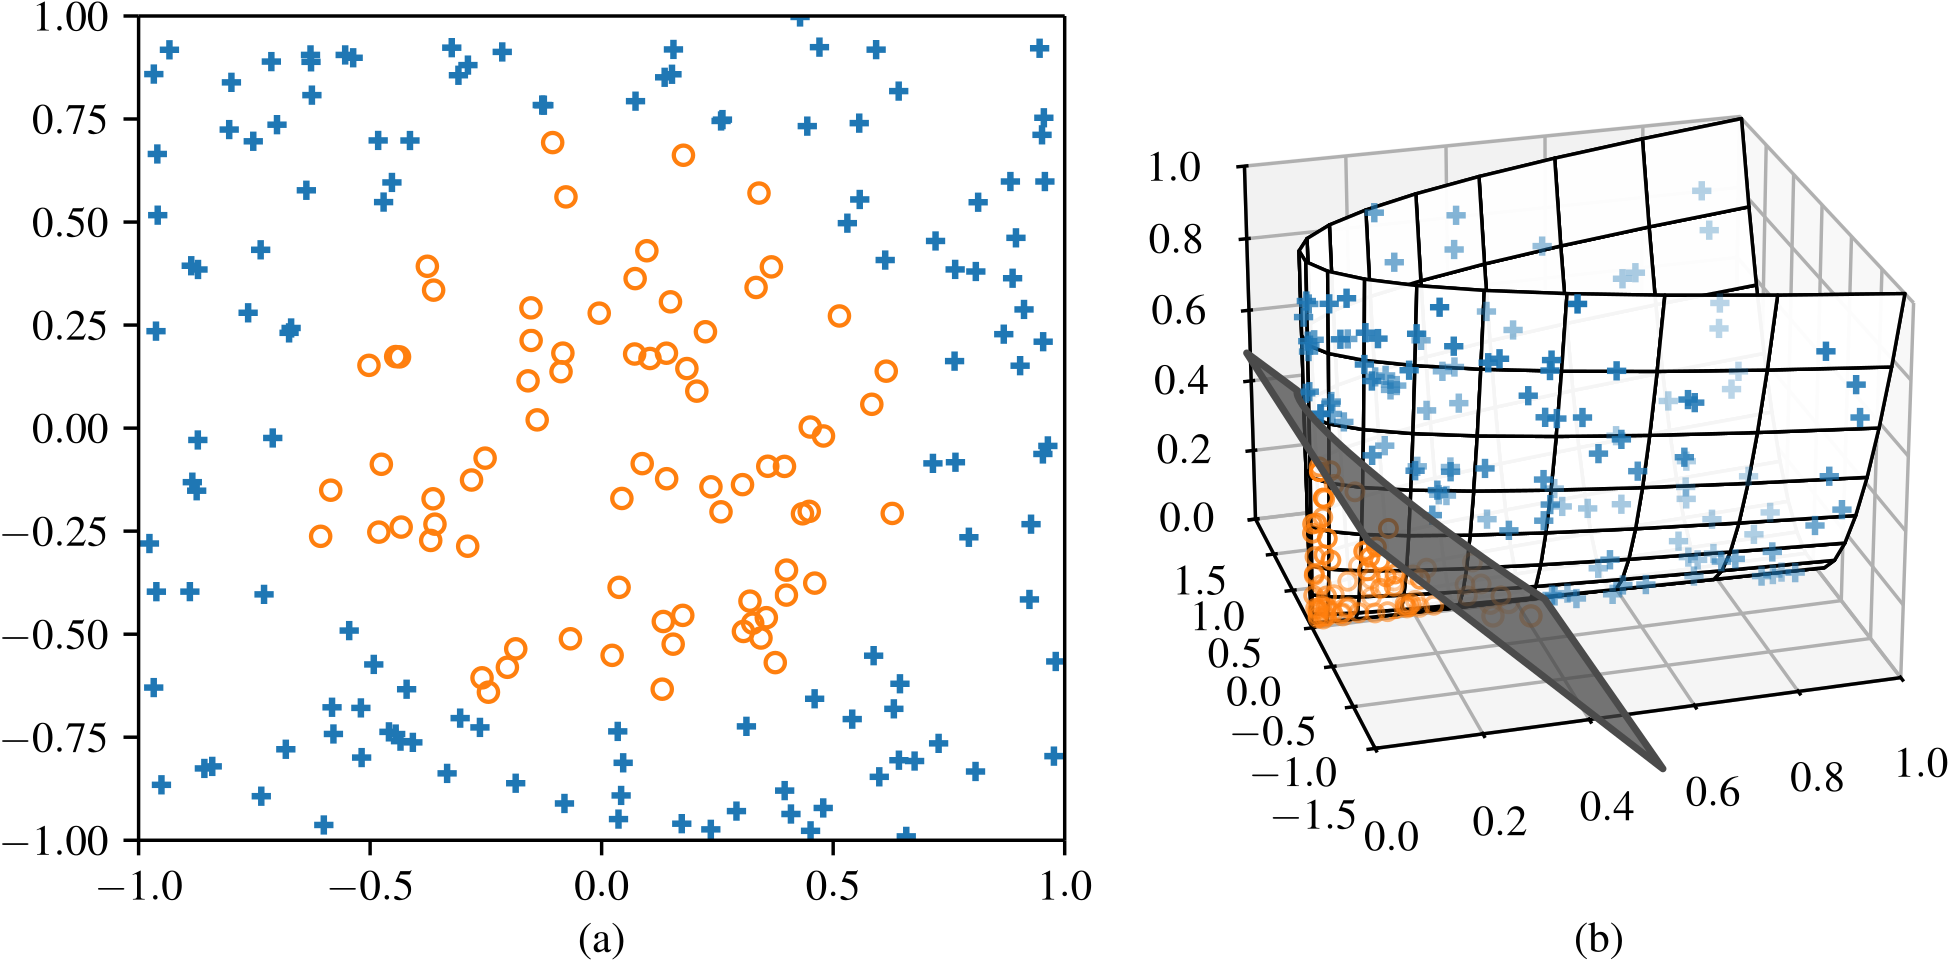
\includegraphics[width=\textwidth]{../figures/SVM_nonlinear_illustration}

\vspace{0.3em}
Nonlinear data transformed to a separable space.

\end{columns}
\end{frame}

%------------------------------------------------

\begin{frame}{Adding Polynomial Features}
\begin{columns}

\column{0.42\textwidth}

A simple feature transformation can make data linearly separable.

\vspace{0.5em}

Example:

\[
x_2 = x_1^2
\]

\vspace{0.5em}

The original one-dimensional data are not separable.

\vspace{0.5em}

After adding \(x_2\), the data become separable in two dimensions.

\column{0.58\textwidth}
\centering
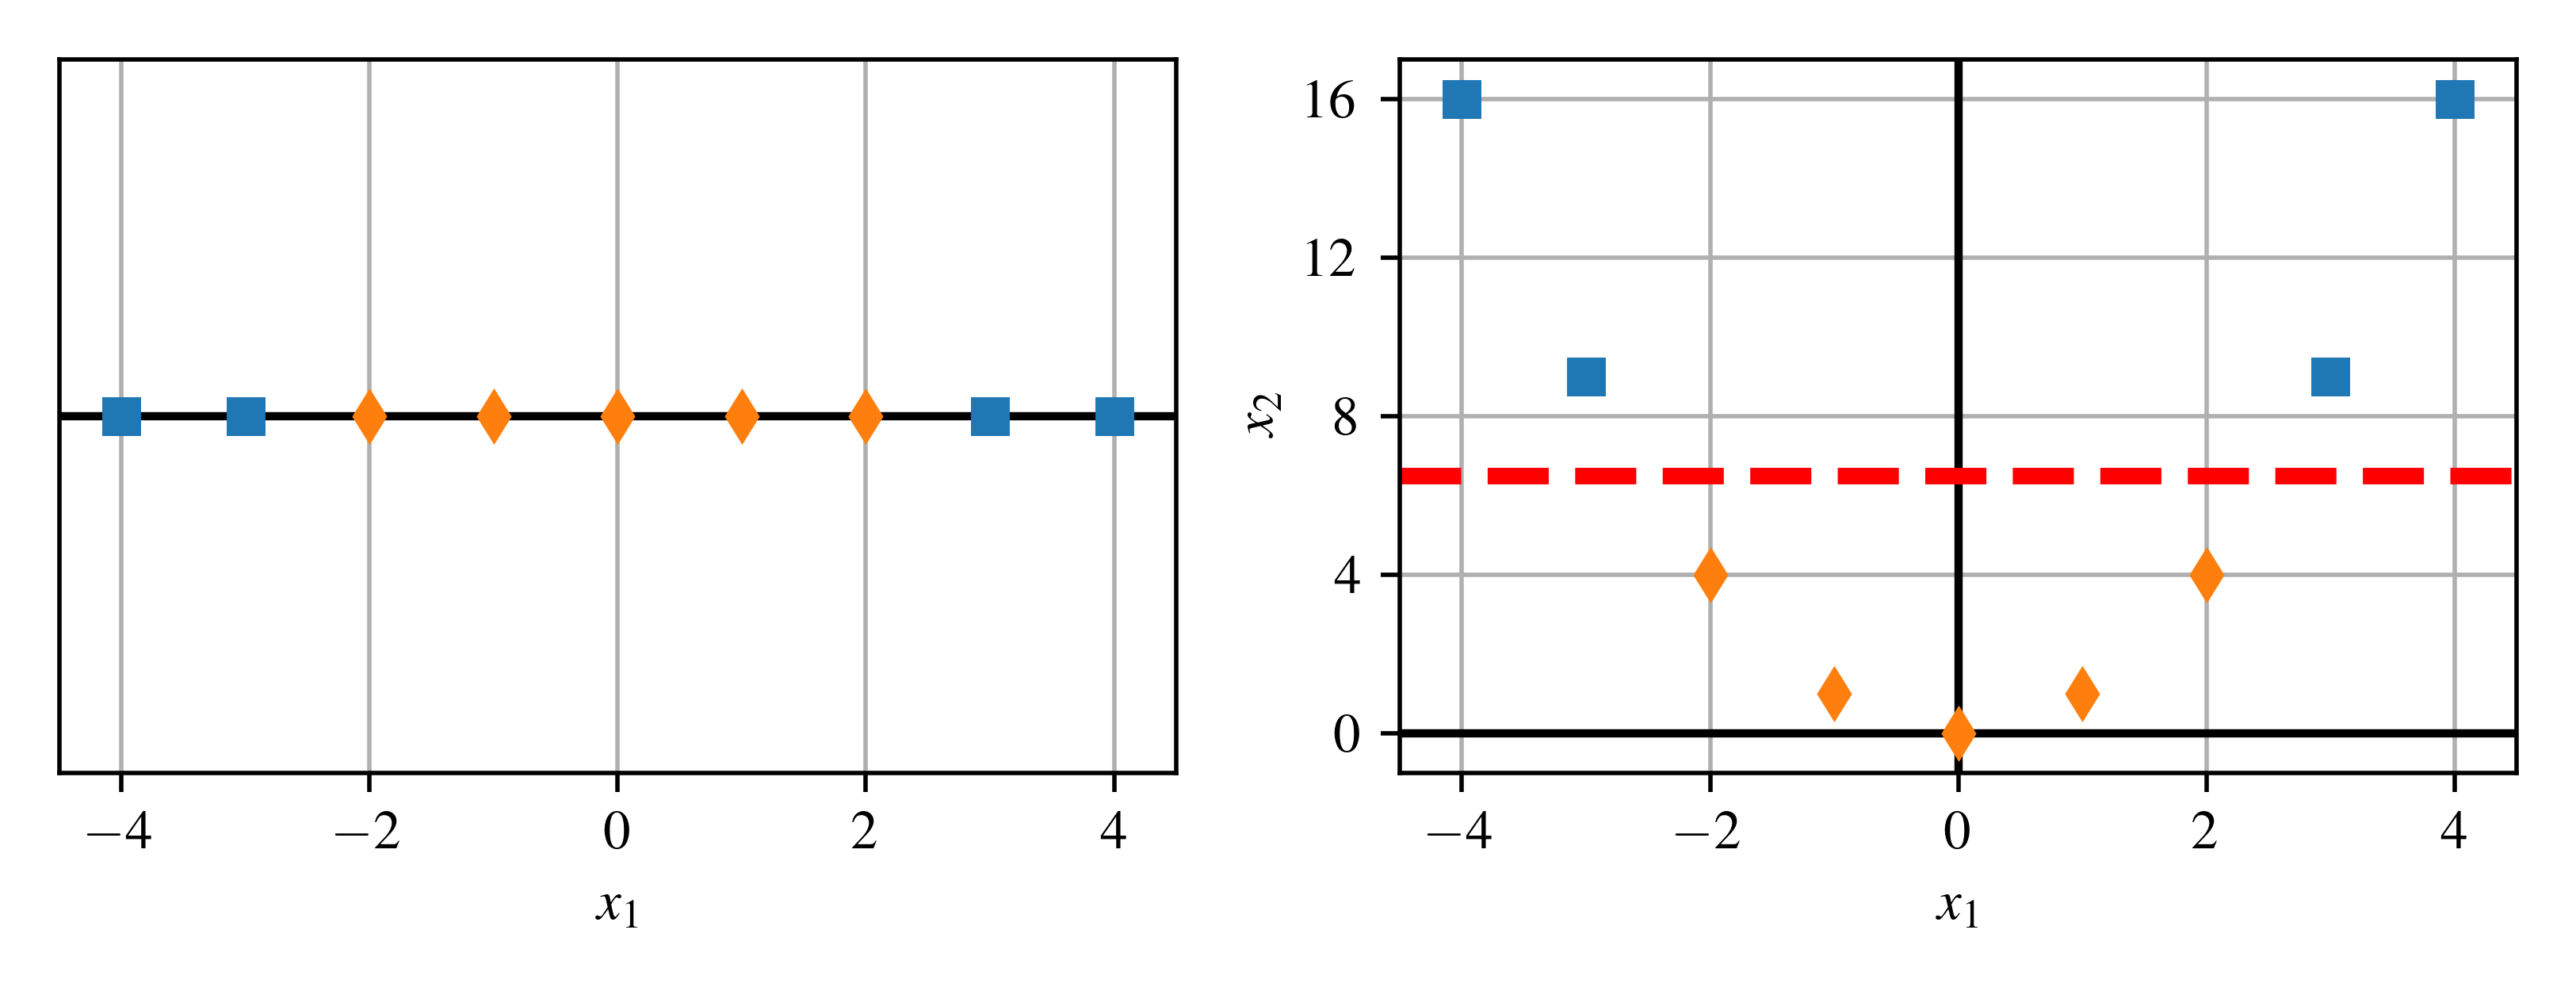
\includegraphics[width=\textwidth]{../figures/SVM_higher_dimensions.png}

\vspace{0.3em}
SVM in higher dimensions.

\end{columns}
\end{frame}

%------------------------------------------------

\begin{frame}{Polynomial Features with LinearSVC}
\begin{columns}

\column{0.42\textwidth}

In Scikit-Learn, this can be implemented with a pipeline:

\vspace{0.5em}

\begin{itemize}
\item \texttt{PolynomialFeatures}
\item \texttt{StandardScaler}
\item \texttt{LinearSVC}
\end{itemize}

\vspace{0.5em}

This works well for datasets like:

\[
\texttt{make\_moons()}
\]

\vspace{0.5em}

The classifier is still linear in the transformed feature space.

\column{0.58\textwidth}
\centering
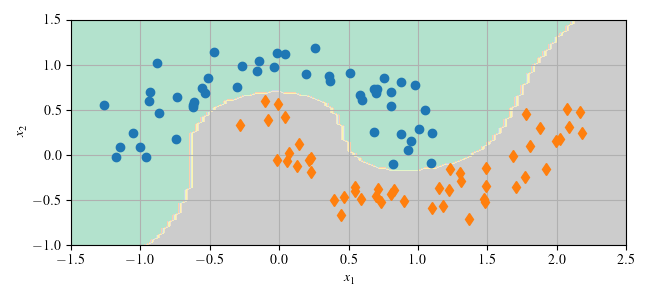
\includegraphics[width=\textwidth]{../figures/SVM_polynomial_features.png}

\vspace{0.3em}
SVM classifier with polynomial features.

\end{columns}
\end{frame}

%------------------------------------------------

\begin{frame}{Example 7.2: Nonlinear Classification}

\begin{itemize}
\item Generate nonlinear data using \texttt{make\_moons}
\item Build a pipeline with:
\begin{itemize}
\item \texttt{PolynomialFeatures}
\item \texttt{StandardScaler}
\item \texttt{LinearSVC}
\end{itemize}

\vspace{0.5em}

\item Train a linear SVM in the expanded feature space
\item Visualize the resulting nonlinear decision boundary
\end{itemize}

\vspace{0.5em}

This example shows how feature transformations can make nonlinear classification possible.

\end{frame}

%------------------------------------------------

\begin{frame}{The Kernel Trick}

Polynomial feature expansion can become expensive.

\vspace{0.5em}

Problems:
\begin{itemize}
\item Low-degree features may underfit
\item High-degree features may create too many variables
\item Computation can become slow
\end{itemize}

\vspace{0.5em}

The kernel trick avoids explicitly expanding the feature space.

\vspace{0.5em}

It replaces:

\[
\mathbf{x}^{\top}\mathbf{z}
\]

with:

\[
k(\mathbf{x},\mathbf{z})
\]

\end{frame}

%------------------------------------------------

\begin{frame}{Kernel Trick Interpretation}

The kernel function

\[
k(\mathbf{x},\mathbf{z})
\]

computes similarity between two data points.

\vspace{0.5em}

It allows the SVM to behave as if it were working in a higher-dimensional feature space.

\vspace{0.5em}

Benefits:

\begin{itemize}
\item Curved decision boundaries
\item No explicit feature expansion
\item Powerful nonlinear classification
\end{itemize}

\vspace{0.5em}

The kernel trick is implemented in:

\[
\texttt{SVC}
\]

\end{frame}

%------------------------------------------------

\begin{frame}{Polynomial Kernel}
\begin{columns}

\column{0.42\textwidth}

A polynomial kernel can produce nonlinear decision boundaries.

\vspace{0.5em}

The degree controls model flexibility.

\vspace{0.5em}

Higher degree:
\begin{itemize}
\item More flexible
\item More risk of overfitting
\end{itemize}

\vspace{0.5em}

The \texttt{coef0} parameter controls the influence of lower- vs. higher-degree terms.

\column{0.58\textwidth}
\centering
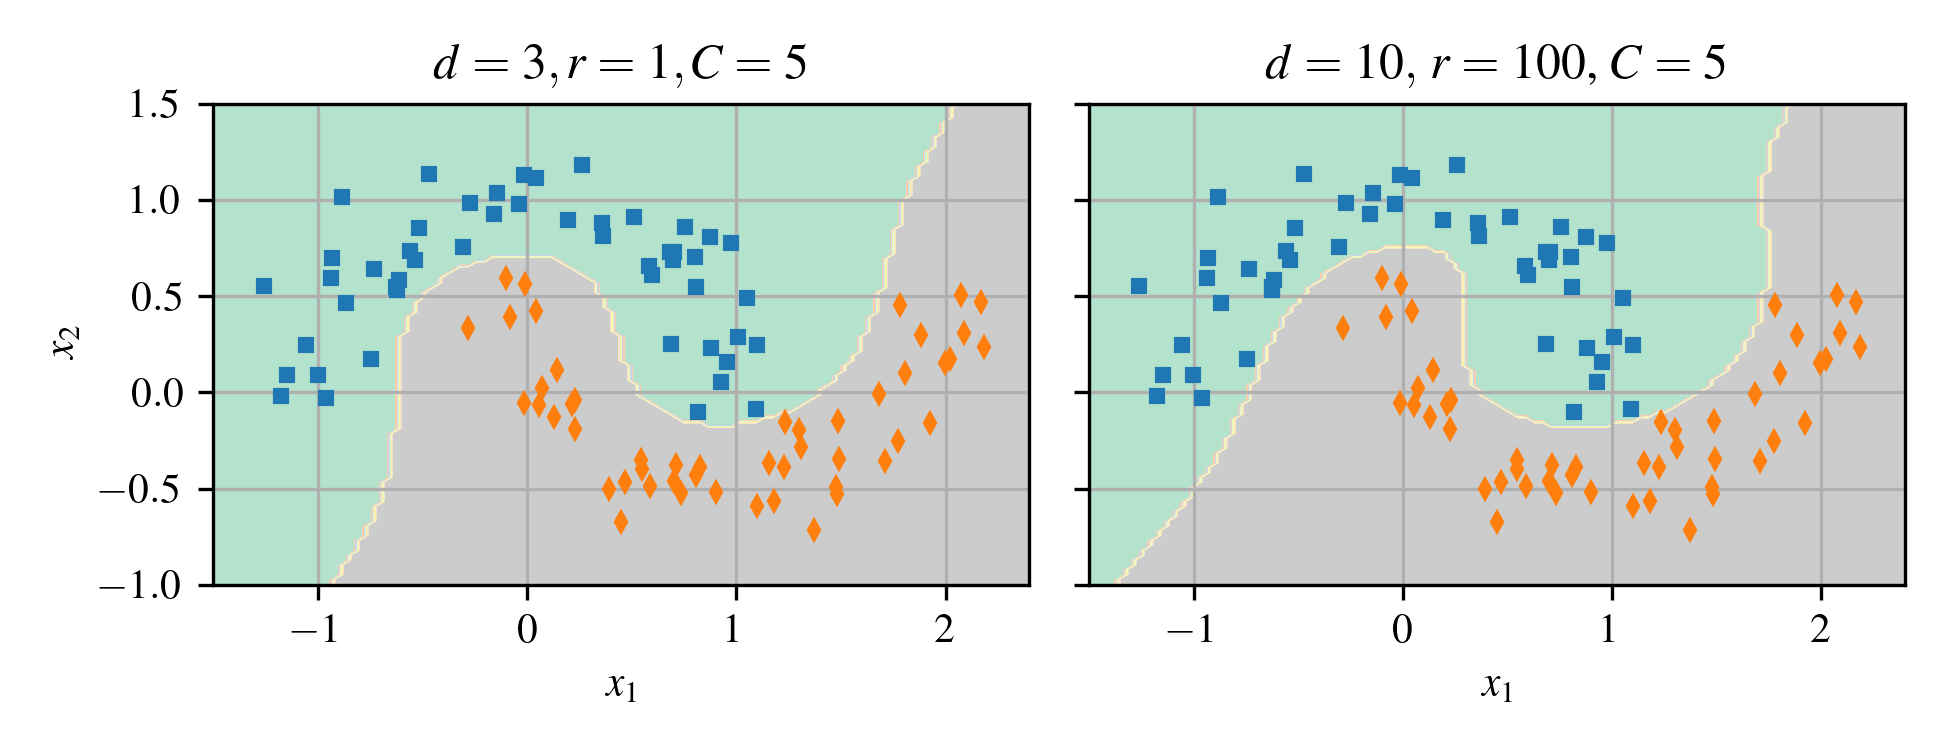
\includegraphics[width=\textwidth]{../figures/SVM_polynomial_kernel.png}

\vspace{0.3em}
Polynomial-kernel SVMs.

\end{columns}
\end{frame}

%------------------------------------------------

\begin{frame}{Tuning Kernel SVMs}

Kernel SVMs can be sensitive to hyperparameters.

\vspace{0.5em}

Common tuning approach:

\begin{itemize}
\item Start with a broad grid search
\item Identify promising regions
\item Refine with a narrower grid search
\end{itemize}

\vspace{0.5em}

Important hyperparameters:

\begin{itemize}
\item \(C\)
\item polynomial degree
\item \texttt{coef0}
\item \(\gamma\) for RBF kernels
\end{itemize}

\vspace{0.5em}

Understanding each hyperparameter helps guide the search.

\end{frame}

%------------------------------------------------

\begin{frame}{Standard Kernels}

Three kernels cover most practical cases.

\vspace{0.5em}

Polynomial kernel:

\[
k_{\text{poly}}(\mathbf{x},\mathbf{z})
=
(\mathbf{x}^{\top}\mathbf{z}+c)^d
\]

\vspace{0.5em}

RBF kernel:

\[
k_{\text{rbf}}(\mathbf{x},\mathbf{z})
=
\exp
\left(
-\gamma
\lVert
\mathbf{x}-\mathbf{z}
\rVert^2
\right)
\]

\vspace{0.5em}

Sigmoid kernel:

\[
k_{\text{sig}}(\mathbf{x},\mathbf{z})
=
\tanh
\left(
\kappa\mathbf{x}^{\top}\mathbf{z}
+
\theta
\right)
\]

\end{frame}

%------------------------------------------------

\begin{frame}{Choosing a Kernel}

A practical rule of thumb:

\vspace{0.5em}

\begin{itemize}
\item Start with the RBF kernel
\item Try polynomial kernels when interaction order matters
\item Treat the sigmoid kernel as experimental
\end{itemize}

\vspace{0.5em}

\begin{exampleblock}{Note}
Kernel methods require scaled features. Standardization is usually important before training.
\end{exampleblock}

\vspace{0.5em}

The best kernel depends on:

\begin{itemize}
\item Dataset size
\item Noise level
\item Feature interactions
\item Desired model flexibility
\end{itemize}

\end{frame}

%------------------------------------------------

\begin{frame}{Example 7.3: Polynomial Kernel Trick}

\begin{itemize}
\item Use \texttt{SVC} instead of \texttt{LinearSVC}
\item Apply a third-degree polynomial kernel
\item Classify nonlinear \texttt{make\_moons} data
\item Use a Scikit-Learn pipeline
\item Visualize the curved decision boundary
\end{itemize}

\vspace{0.5em}

This example shows how the kernel trick produces nonlinear classification without explicitly building polynomial features.

\end{frame}

%------------------------------------------------

\section{7.3~Computational Complexity}
\begin{frame}{Computational Complexity}

Scikit-Learn provides several SVM-related classifiers.

\vspace{0.5em}

\begin{center}
\resizebox{\textwidth}{!}{
\begin{tabular}{llll}
\hline
class & time complexity & out-of-core & kernel trick \\ \hline
\texttt{LinearSVC} & \(O(mn)\) & no & no \\
\texttt{SVC} & \(O(m^2n)\) to \(O(m^3n)\) & no & yes \\
\texttt{SGDClassifier} & \(O(mn)\) & yes & no \\ \hline
\end{tabular}
}
\end{center}

\vspace{0.5em}

Scaling is required for all three methods.

\end{frame}

%------------------------------------------------

\begin{frame}{LinearSVC vs. SVC}

\texttt{LinearSVC}

\begin{itemize}
\item Uses \texttt{liblinear}
\item Linear decision boundary only
\item Scales approximately as \(O(mn)\)
\item Good for large, high-dimensional datasets
\end{itemize}

\vspace{0.5em}

\texttt{SVC}

\begin{itemize}
\item Uses \texttt{libsvm}
\item Supports kernels
\item Can model nonlinear boundaries
\item Slower for large datasets
\end{itemize}

\end{frame}

%------------------------------------------------

\section{7.4~SVM Regression}
\begin{frame}{Support Vector Regression}

Support Vector Regression adapts SVMs to continuous outputs.

\vspace{0.5em}

Instead of separating classes, SVR fits a prediction curve surrounded by a tube.

\vspace{0.5em}

Tube width:

\[
\epsilon
\]

\vspace{0.5em}

Points inside the tube do not affect the loss.

\vspace{0.5em}

The regularization parameter \(C\) controls how strongly violations outside the tube are penalized.

\end{frame}

%------------------------------------------------

\begin{frame}{Linear SVR}
\begin{columns}

\column{0.42\textwidth}

Linear SVR fits a linear function with an \(\epsilon\)-insensitive margin.

\vspace{0.5em}

Larger \(\epsilon\):
\begin{itemize}
\item Wider tube
\item More tolerance
\end{itemize}

\vspace{0.5em}

Smaller \(\epsilon\):
\begin{itemize}
\item Narrower tube
\item More sensitive fit
\end{itemize}

\column{0.58\textwidth}
\centering
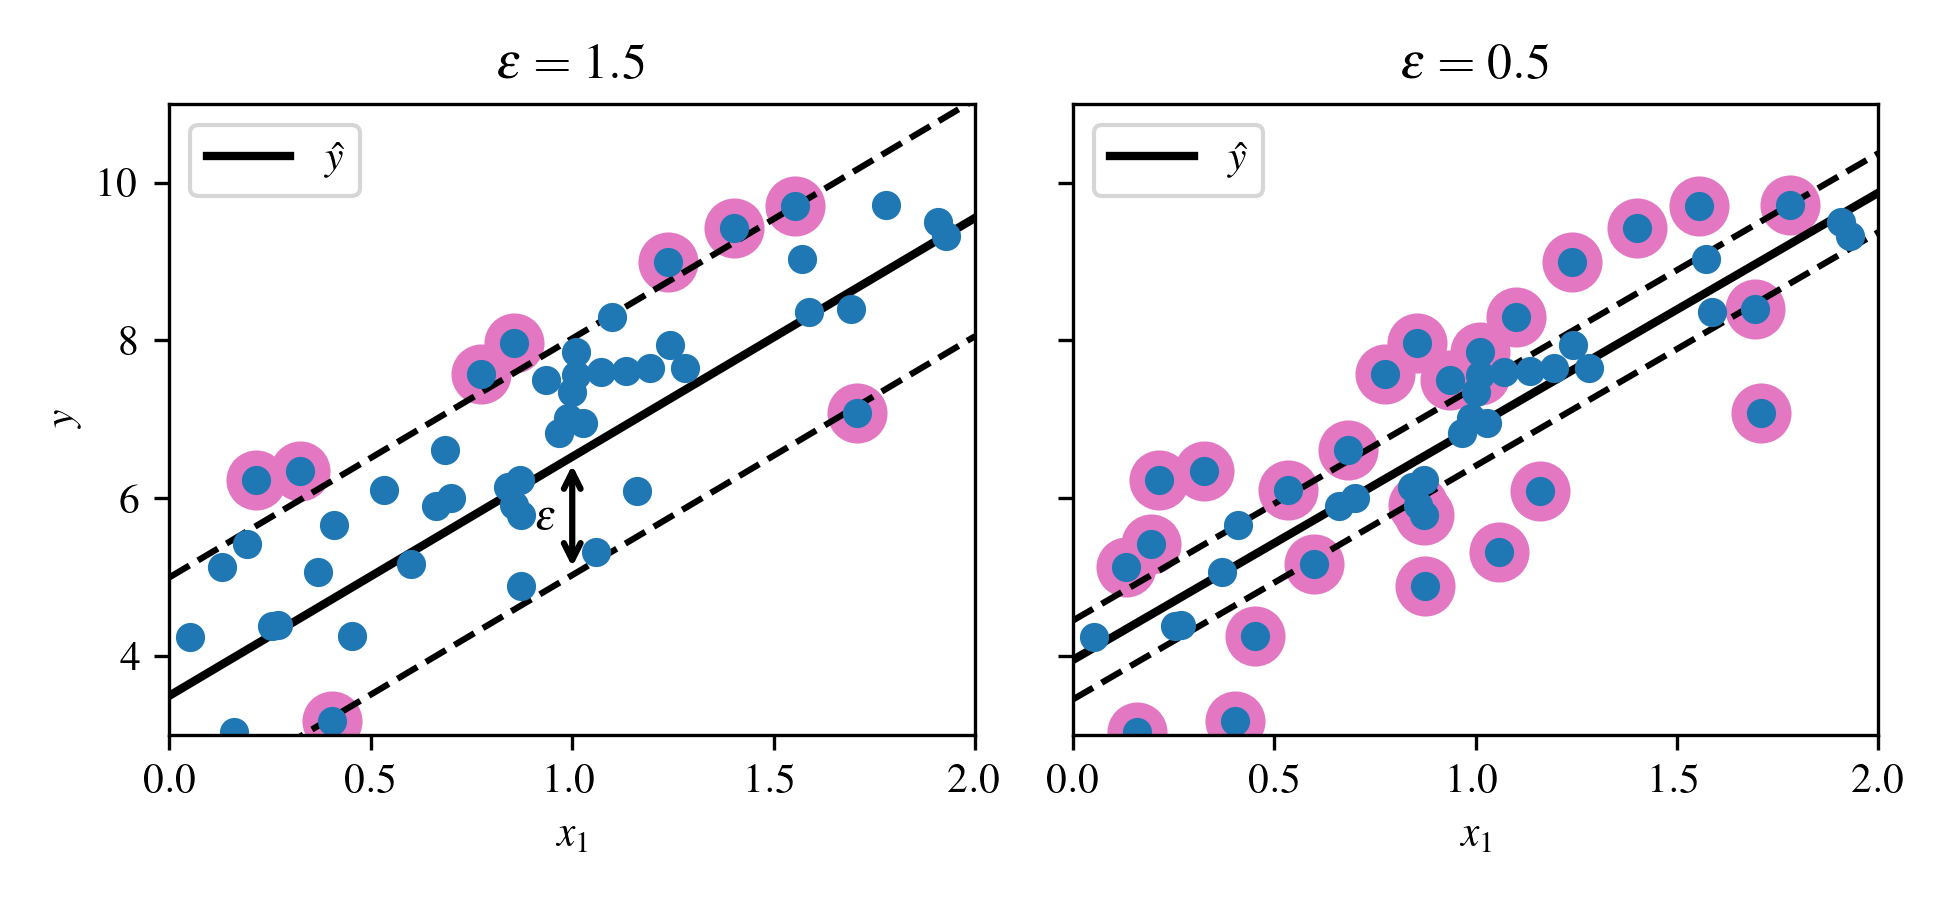
\includegraphics[width=\textwidth]{../figures/SVM_Regression.png}

\vspace{0.3em}
Linear SVR with different \(\epsilon\) values.

\end{columns}
\end{frame}

%------------------------------------------------

\begin{frame}{Kernel SVR}

When the relationship is nonlinear, SVR can use kernels.

\vspace{0.5em}

Prediction function:

\[
f(x)
=
\sum_{i=1}^{m}
(\alpha_i-\alpha_i^{*})
k(x_i,x)
+
b
\]

\vspace{0.5em}

Common kernels:

\begin{itemize}
\item RBF
\item Polynomial
\end{itemize}

\vspace{0.5em}

Kernel SVR is powerful for small to medium datasets but can become slow as the dataset grows.

\end{frame}

%------------------------------------------------

\begin{frame}{Polynomial SVR}
\begin{columns}

\column{0.42\textwidth}

A polynomial kernel can model nonlinear regression behavior.

\vspace{0.5em}

The parameter \(C\) controls regularization.

\vspace{0.5em}

Larger \(C\):
\begin{itemize}
\item Less regularization
\item Tighter fit
\end{itemize}

\vspace{0.5em}

Smaller \(C\):
\begin{itemize}
\item More regularization
\item Smoother fit
\end{itemize}

\column{0.58\textwidth}
\centering

\includegraphics[width=\textwidth]{../figures/SVM_regression_2nd_degree.png}

\vspace{0.3em}
Polynomial-kernel SVR.

\end{columns}
\end{frame}

%------------------------------------------------

\begin{frame}{Example 7.4: SVM Polynomial Regression}

\begin{itemize}
\item Fit noisy quadratic data using SVR
\item Use a polynomial kernel
\item Introduce an \(\epsilon\)-insensitive margin
\item Visualize the regression curve and tolerance region
\end{itemize}

\vspace{0.5em}

This example demonstrates how SVR can model nonlinear relationships while controlling how closely the model follows the data.

\end{frame}






\end{document}




